\section{Experimental Evaluation} %\label{sec:extension_experiments}

\subsection{Kd-tree versus quadtree performance} \label{sec:comparison}
In order to compare the quadtree and the kd-tree partition strategies we analyze their performance during the construction of the spatial data structure which defines the cells that the partition will use based on the sample, the cost of partitioning; populating the cells with the full datasets, and the overall time to complete the phases of the overlay operation using each partitioning approach.  We use the datasets of MainUS and GADM described in Table \ref{tab:datasets}.

 \begin{figure}
     \centering
     \begin{tabular}{cc}
         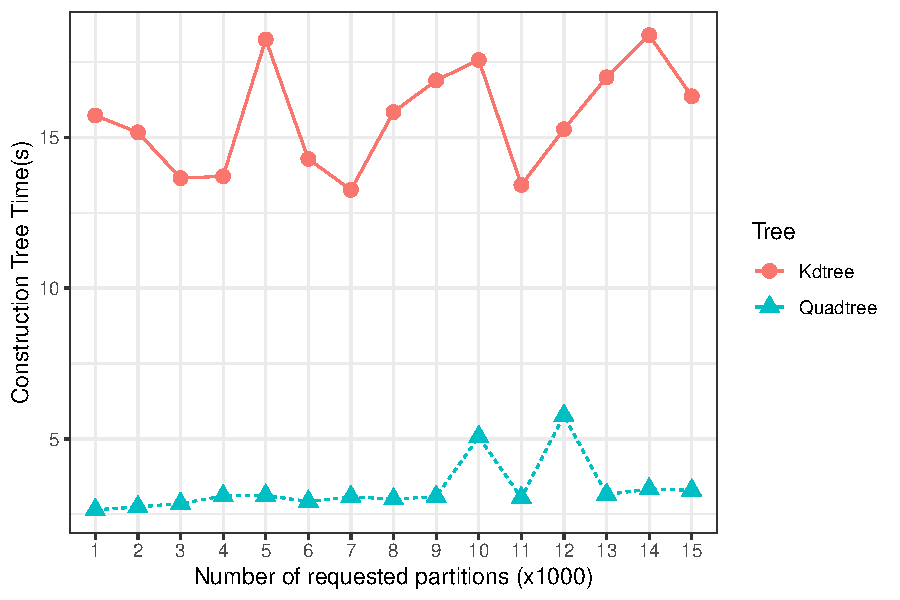
\includegraphics[width=0.49\linewidth]{chapterSDCEL/K_Creation_US.pdf} & 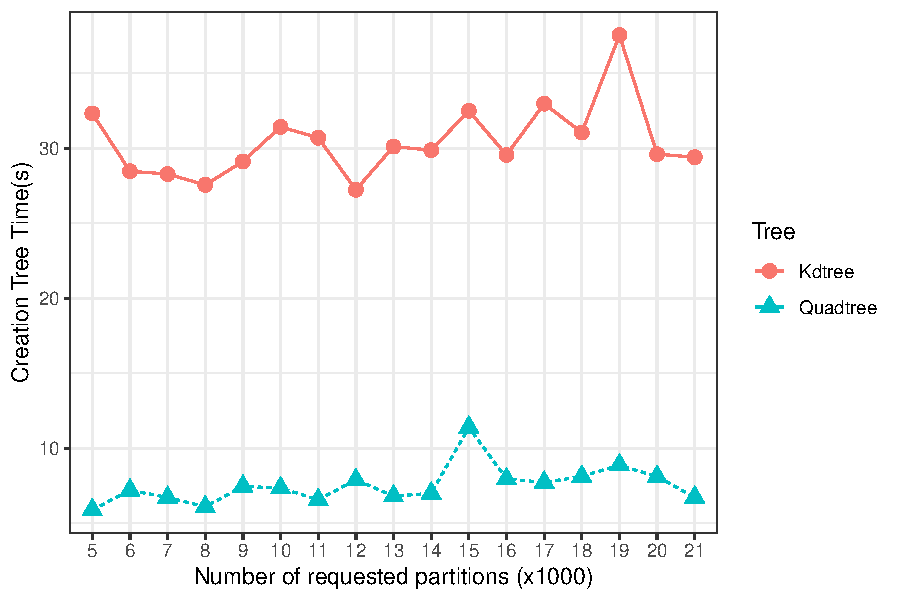
\includegraphics[width=0.49\linewidth]{chapterSDCEL/K_Creation_GADM.pdf} \\
         (a) & (b)
     \end{tabular}
     \caption{Construction time for the spatial data structure in the (a) MainUS and (b) GADM datasets.} \label{fig:k_creation_us}
 \end{figure}

 \begin{figure}
     \centering
     \begin{tabular}{cc}
         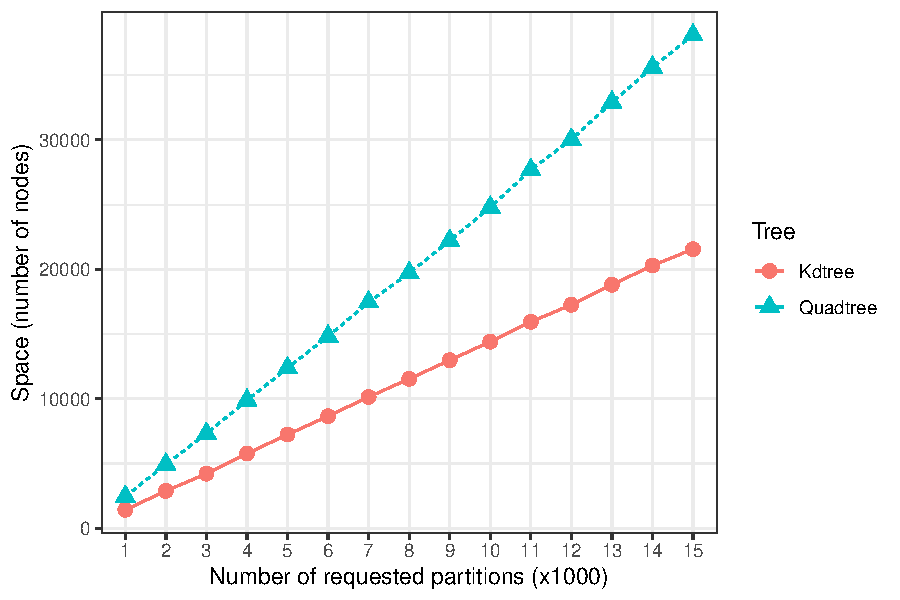
\includegraphics[width=0.49\linewidth]{chapterSDCEL/K_Space_US.pdf} & 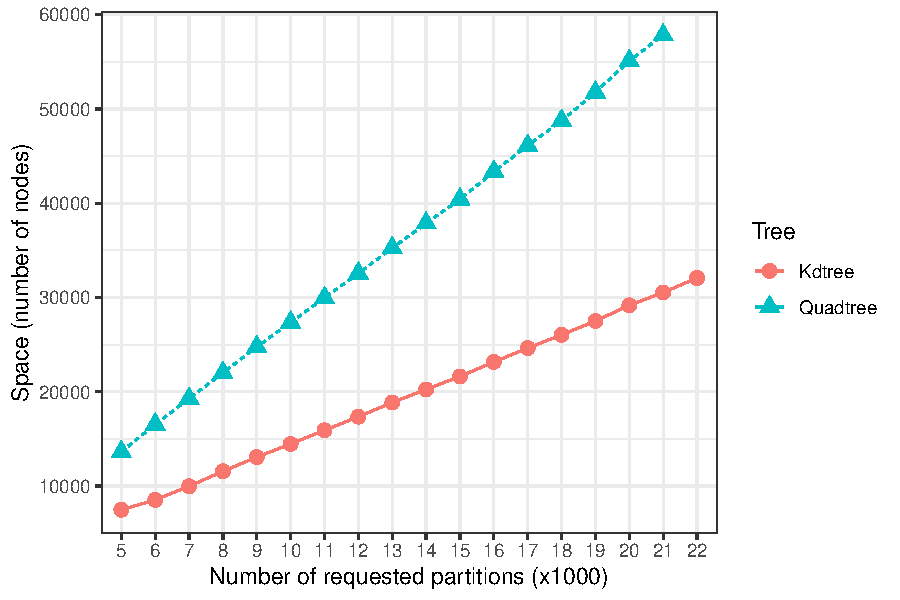
\includegraphics[width=0.49\linewidth]{chapterSDCEL/K_Space_GADM.pdf} \\
         (a) & (b)
     \end{tabular}
     \caption{Number of cells created by each spatial data structure in the (a) MainUS and (b) GADM datasets.} \label{fig:k_space_us}
 \end{figure}

Figure \ref{fig:k_creation_us} depicts the construction time during the sampling of the input layers and the generation of the partitioning cells after requesting a different number of divisions. We can see that the kd-tree takes more time, particularly because of the sorting done at each split, so as to organize the data and localize the middle point. In average, Quadtree takes 23.13\% the time it takes for Kdtree to be created (21.55\% in MainUS and 24.72\% in GADM). However, the Kdtree creation is just 5.86\% of the overall time during the total DCEL construction (6.88\% in MainUS and 4.87\% in GADM).

 \begin{figure}
     \centering
     \begin{tabular}{cc}
         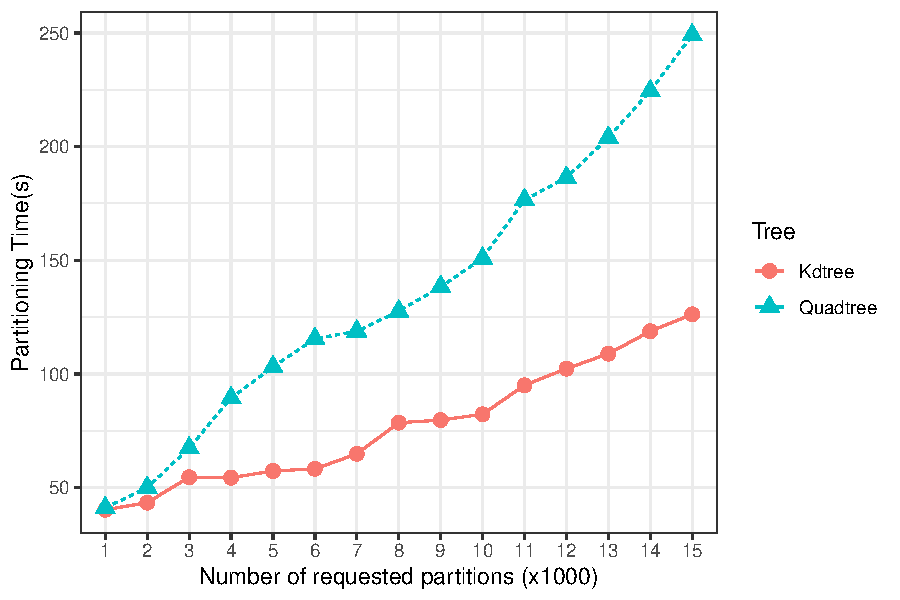
\includegraphics[width=0.49\linewidth]{chapterSDCEL/K_Partitioning_US.pdf} &
         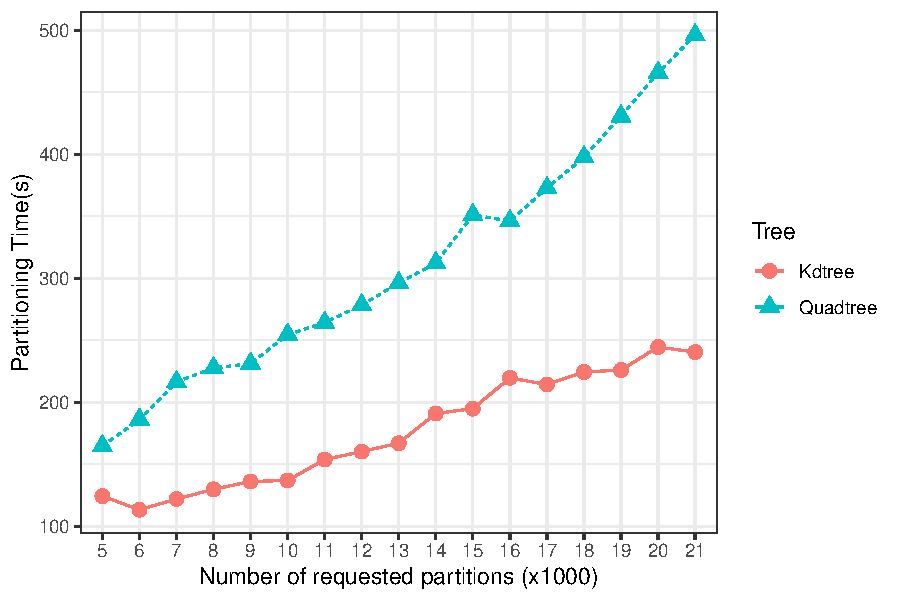
\includegraphics[width=0.49\linewidth]{chapterSDCEL/K_Partitioning_GADM.pdf} \\
         (a) & (b)
     \end{tabular}
     \caption{Data partitioning time using a spatial data structure (a) in the MainUS dataset and (b) in the GADM dataset.} \label{fig:k_partitioning_us}
 \end{figure}

An important characteristic of the behavior of each partitioning scheme is the number of cells (partitions) each sample data structure creates. Figure \ref{fig:k_space_us} depicts the number of cells created by each spatial data structure. As the quadtree follows a space-oriented technique, it creates more nodes (4 at each split) and thus generates more leaves (cells); more of them are prone to be empty compared to the kd-tree.

Figure \ref{fig:k_partitioning_us} shows the cost to partition the full content of both layers. Given a sample tree data structure, each edge is assigned to a cell (partition) depending on which leaf the edge is located; edges are assigned (copied) to all leaves they intersect. Then, a shuffle operation is performed to move the data to the corresponding node that will handle this cell (partition). This figure shows that the quadtree partitioning takes more time. This depends largely on the number of leaves created by the sample tree and the number of edges that overlap partitions (which is expected to be larger for the quadtree since it uses more and thus smaller cells).

\begin{figure}
    \centering
    \begin{tabular}{cc}
        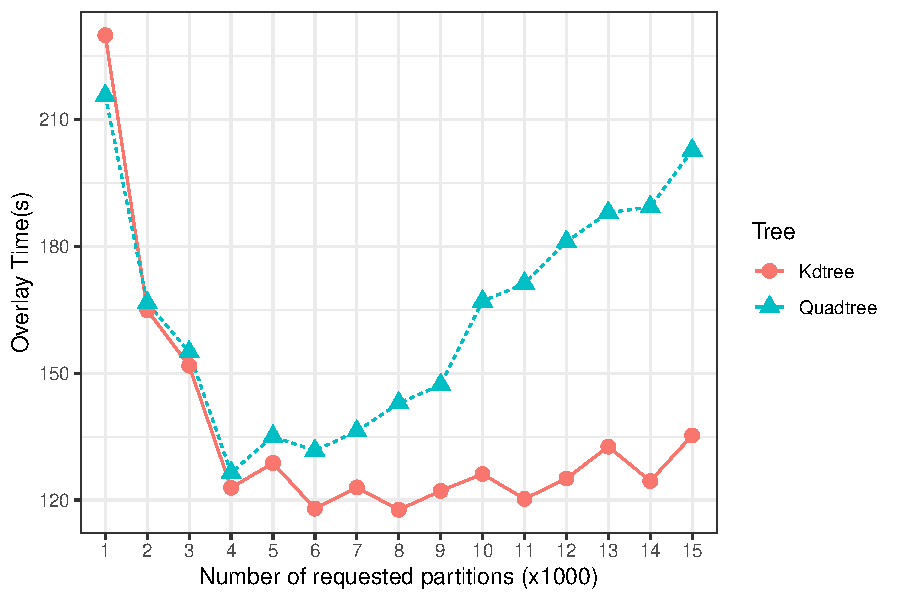
\includegraphics[width=0.49\linewidth]{chapterSDCEL/K_Overlay_US.pdf} &
        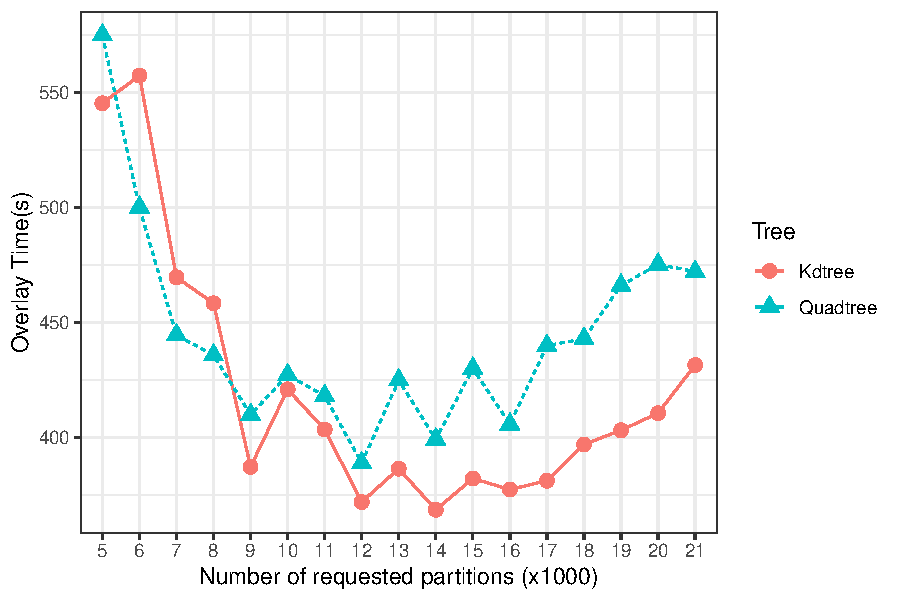
\includegraphics[width=0.49\linewidth]{chapterSDCEL/K_Overlay_GADM.pdf} \\
        (a) & (b)
    \end{tabular}
    \caption{Execution time for the overlay operation using a spatial data structure in the MainUS (a)and GADM (b) dataset.} \label{fig:k_overlay_us}
\end{figure}

Once the data is assigned to their partitions, the overlay operation can be executed.  Figure \ref{fig:k_overlay_us} shows the overlay performance under each partition strategy, for different number of cells. The Kd-tree approach performs better; as the quadtree tends to generate more and emptier cells, its performance is directly affected.

As it was said before, in particular on partitioning based on Kdtree, the smaller number of cells/partitions used in this approach give also an improvement on the impact of shuffling during the partition strategy because the number and size of the resulting partitions have a lower impact into the communication cost.

Finally, we consider the speed-up and scale-up performance using the kd-tree partitioning. Figure \ref{fig:k_scale_speed_us}(a) shows the speed-up performance using the MainUS dataset (36M edges) while varying the number of nodes (for 3, 6, and 12 nodes). Similar to the quadtree partitioning strategy, the kd-tree partitioning shows good speed-up performance. As resources duplicate the execution time improves almost by a half.

Figure \ref{fig:k_scale_speed_us}(b) shows the scale-up performance of the kd-tree partitioning approach. We followed the same procedure described in Section \ref{sec:speed_scale} to generate datasets for 8M, 16M, and 32M edges from the MainUS dataset and ran the kd-tree partitioning strategy with 3, 6, and 12 nodes, respectively. Again the kd-tree partitioning shows good speed-up performance, which remains flat as the load per node is almost equal.

\begin{figure}
    \centering
    \begin{tabular}{cc}
        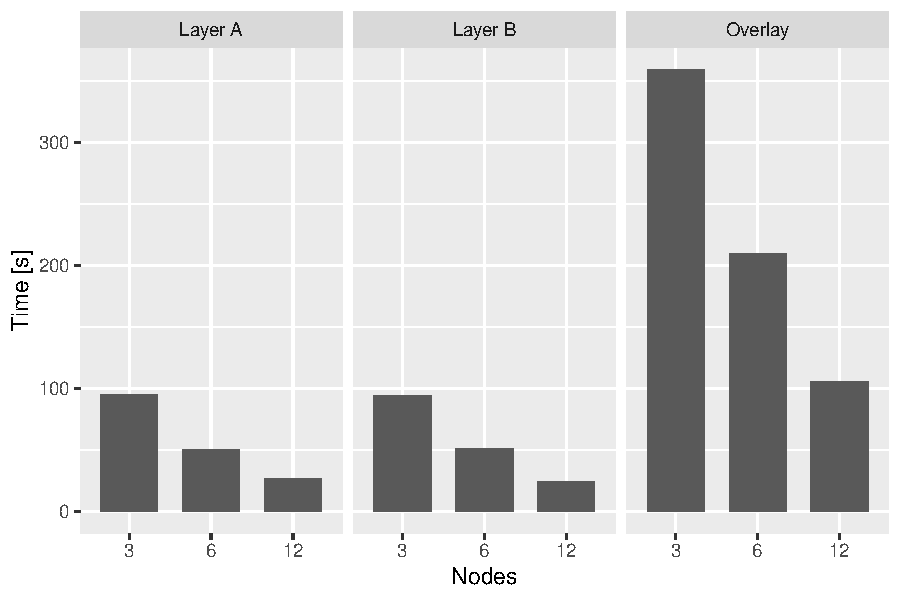
\includegraphics[width=0.49\linewidth]{chapterSDCEL/US_speedup.pdf} & 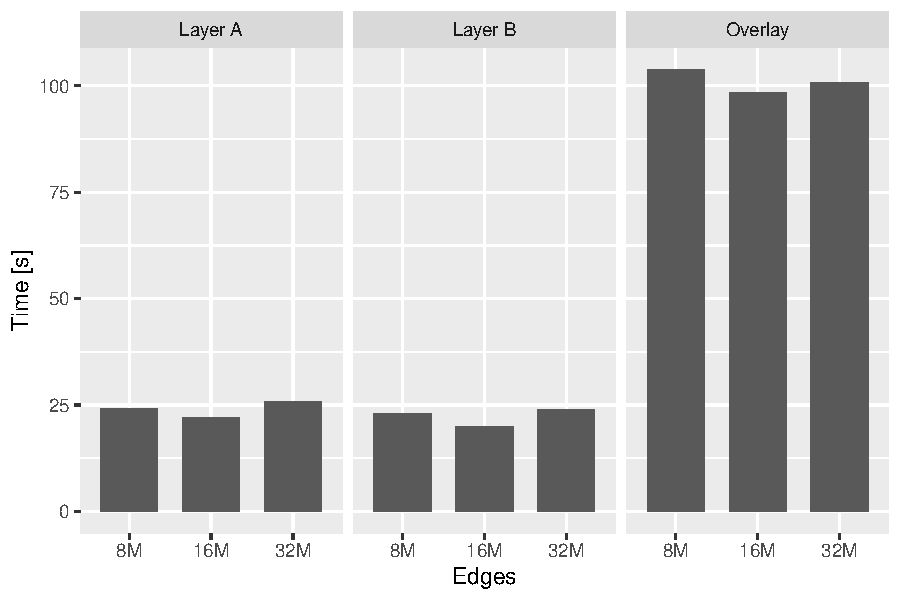
\includegraphics[width=0.49\linewidth]{chapterSDCEL/US_scaleup.pdf} \\
        (a) & (b)
    \end{tabular}
    \caption{(a)Speed Up and (b) Scale Up performance of the Kdtree partitioning using the MainUS dataset.} \label{fig:k_scale_speed_us}
\end{figure}

%% Extension
\subsection{Overlaying Polygons with Dangle and Cut Edges}
\begin{table}
    \caption{Overlaying Polygons with Dangle and Cut Edges Dataset}
    \label{tab:dangles}
    \begin{tabular}{c c c c}
        \toprule
        Dataset & Number Layer $A$ of Polygons & Number of Layer $B$ Edges & Result Polygons \\
        \midrule
        TN & 1,272 & 3,380,780 & 41,761 \\
        GA & 1,633 & 4,647,171 & 49,125 \\
        NC & 1,272 & 7,212,604 & 22,413 \\
        TX & 4,399  & 8,682,950 & 98,635 \\
        VA & 1,554 & 8,977,361 & 38,941 \\
        CA & 7,038 & 9,103,610 & 96,916\\
        \bottomrule
    \end{tabular}
\end{table}

\begin{figure}
    \centering
    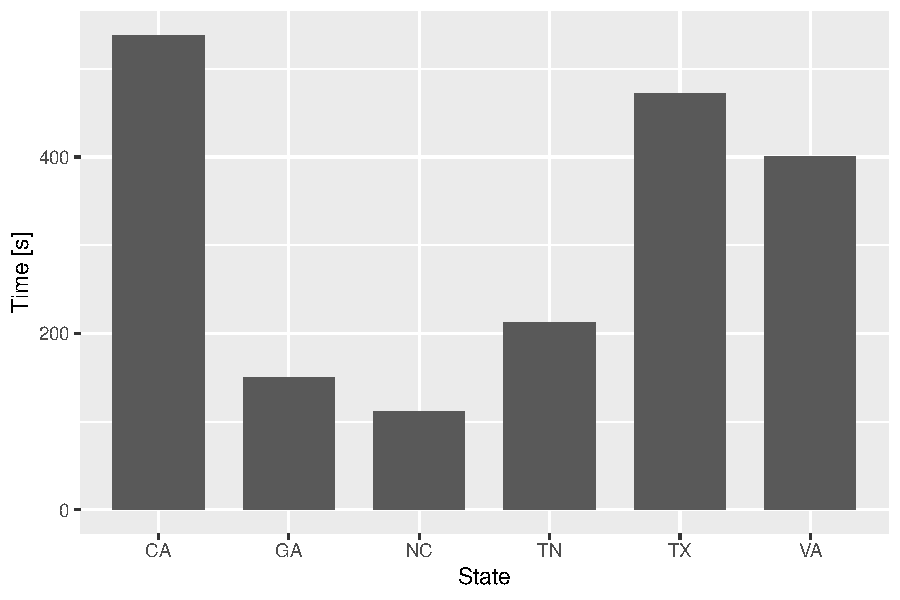
\includegraphics[width=0.7\linewidth]{chapterSDCEL/states.pdf}
    \caption{Overlaying State polygons with dangle and cut edges.}
    \label{fig:dangle}
\end{figure}

%\ref{sec:over_dang}
In this section, we examine the performance of overlaying polygons with dangle and cut edges resulting from the polygonization as detailed in \textcolor{red}{Section XX}.  Table \ref{tab:dangles} shows the number of polygons for each state for the first layer of the overlay. It also shows the number of dangle and cut edges per state for the second layer of the overlay. Finally, it shows the number of resultant polygons per state.  From Figure \ref{fig:dangle}, we conclude that the running time is affected by the number of dangle and cut edges and the number of intersections between the two layers (represented by the number of generated polygons).  TN and GA have a relatively smaller number of dangle and cut edges, so they have lower execution times compared to VA, TX, and CA. However, since the intersections in NC are significantly less than those of TN and GA, NC has the lowest execution time. TX, VA, and CA have a comparable number of edges; however, VA has the least number of intersections, resulting in lower execution time compared to TX and CA.
